\documentclass[a4paper,12pt]{article}

\usepackage{url}
\usepackage{amsmath}
\usepackage{amssymb}
\usepackage{epsfig}
\usepackage{mathtools}
\usepackage{graphics}
\usepackage{fancyhdr}
\usepackage{cite}
\usepackage{algorithm}
\usepackage[noend]{algpseudocode}

\usepackage{color}
\usepackage{colortbl}
\definecolor{LightGray}{gray}{0.9}

\graphicspath{{pictures/}}

\title{Report for assignment 2 in the course DD2438 at KTH}
\author{\hspace*{-0.5cm}
GROUP10\\
\begin{tabular}{cccc}
Arash Safari & Ermias Gebremeskel \\
%BIRTHDATE1 & BIRTHDATE2 \\
asafari@kth.se & ermiasg@kth.se \\
%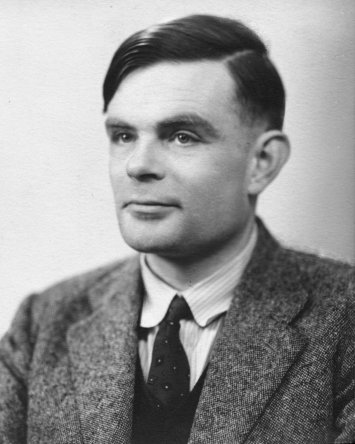
\includegraphics[width=0.13\linewidth]{Alan_Turing_photo} & 
%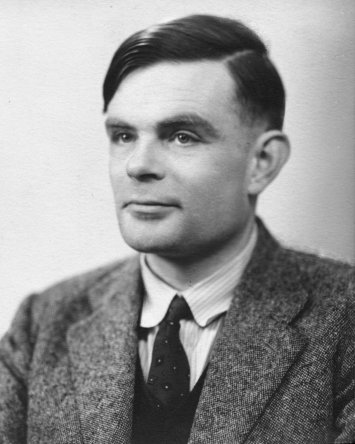
\includegraphics[width=0.13\linewidth]{Alan_Turing_photo}
\end{tabular}} 
\date{}

\pagestyle{fancy}
\setlength{\headheight}{15pt}
\fancyhf{}
\lhead{DD2438 agent16} % DO NOT REMOVE!!!!
\rhead{Arash Safari, Ermias Gebremeskel} %% UPDATE WITH YOUR NAMES
\begin{document}

\maketitle
\thispagestyle{fancy}

\begin{abstract}
This paper will discuss autonomous system motion models including path following and path planing algorithms for these models. This is done by researching and implementing four motion models to simulate the movement of objects in a frictionless two dimensional space and then find a working path following and planing algorithms for these models. The final implementation includes motion models for discrete, kinematic (point and car), dynamic (point and car), and differential drive, with a simple path finding algorithm that takes two points (start and target) and attempt to steer an object to its target. The paths for the models were manly constructed using two algorithms: visibility graphs and rapidly exploring random tree (RRT). Visibility graph was shown to perform better for the models with only two dimensions (x and y), only being outperformed by RRT when extra dimensions are involved.  
 
\end{abstract}



\clearpage

%%%%%%%%%%%%%%%%%%%%%%%%%%%%%%%%%%%%%%%%%%%%%%%%%%%%%%%%%%%%%
%%%%%%%%%%%%%%%%%%%%%%%%%%%%%%%%%%%%%%%%%%%%%%%%%%%%%%%%%%%%%
\section{Introduction}
\label{sec:intro}

One of the most fundamental cornerstones of autonomous mobile robots is navigation. It is after all perfectly reasonable to expect a 'mobile' robot to be mobile. Unfortunately, it is not always simple to guarantee this feature. Different units with different physical properties move under different constraints. And the interaction with obstacles in the environment introduces an additional level of complexity. Even though this field is rather well explored, and great advances has been made to the point where self-driving cars already is a reality, there still is room for improvement. In this report, we will describe our work done during the first assignment of the DD2438 course, which mainly focuses on navigation of units with varying properties in an obstacle filled area. The purpose of this assignment is to gain an understanding of the theory by studying and implementing existing algorithms and methods.

More specifically, the work that the report describes focuses on generating a path through the obstacle filled area that the unit could follow. This is referred to as 'Path Planning' and is achieved through various algorithms such as Visibility graphs and RRT, which we will describe and compare in detail during the report. The nature and complexity of these generated paths are dependent on the motion model of the units, which is a term for describing the limitation of which the unit was allowed manoeuvre under. The motion models that were explored in this assignment were Discrete, Kinematic and dynamic point models, differential drive model, and Kinematic and Dynamic car models. All of which will be described in more detail in the following chapters. The area that the units needed to navigate through contained non-convex polygon-shaped obstacles. 

\subsection{Contribution} 
 This project is done as an assignment in an introductory course in robotics and does not consist of any real contribution to the field of robotics. Most of the algorithms used in this report are simplifications of already well known and established algorithms. 
The report will however, hopefully be useful to any novice in the field seeking an insight into math and motion planning with multiple agents.   

\subsection{Outline}
In the Section~\ref{sec:relwork},we will describe the related work that we consulted during the execution of the project. The project itself consists of solving three different problems, which are described together with the attempted solutions in the Section~\ref{sec:method}. The experimental setup, as well as details about the experiments themselves can be found in Section~\ref{sec:exps}. And finally, a short summary of the report is given in the Section~\ref{sec:summary}.
 

%%%%%%%%%%%%%%%%%%%%%%%%%%%%%%%%%%%%%%%%%%%%%%%%%%%%%%%%%%%%%
%%%%%%%%%%%%%%%%%%%%%%%%%%%%%%%%%%%%%%%%%%%%%%%%%%%%%%%%%%%%%

\section{Related work}
\label{sec:relwork}
In this Section, the theoretical back ground needed to understand this paper and a short description of few related works that we found useful before and during the implementation of our solutions are discussed.
\subsection{}
\label{sec:mm}

\subsection{Visibility Graphs} 
\label{sec:vg}
The visibility graph\cite{berg_visibility_2000} in the Euclidean plane with polygon obstacle is a graph whose nodes corresponds to the corners of the polygon, and whose edges connect the nodes that can be reached with out crossing a polygon. The visibility graph can then be used to find an optimal path with a graph search algorithm. Visibility graphs are efficient for point models, but for models with higher degree of freedom they do not scale. 

 
\subsection{Rapidly-exploring Random Trees} 
\label{sec:rrt}
Rapidly-exploring Random Trees \cite{lavalle1998rapidly} is an incremental method to quickly explore an entire system of configuration of a model. RRT do not produce an optimal solution but because they can find random path very quickly we can run them multiple times to fine a better path.  

\subsection{}
\label{sec:pp}

%%%%%%%%%%%%%%%%%%%%%%%%%%%%%%%%%%%%%%%%%%%%%%%%%%%%%%%%%%%%%
%%%%%%%%%%%%%%%%%%%%%%%%%%%%%%%%%%%%%%%%%%%%%%%%%%%%%%%%%%%%%
\section{Implementation}
\label{sec:method}
The project consisted of three different parts: "Formation keeping", "Vehicle Routing Problem" and "Collision Avoidance". In this section, each of these problems and the attempted solutions will be covered.  
\subsection{Formation keeping}
\label{sec:mmImpl}
In this problem, the agents are placed in predetermined locations and need to enter a formation as fast as possible. Variations of this problem included:
A) Enter formation with global knowledge of the position of other agents.
B) Enter formation with local knowledge of the position of other agents.
C) Enter a moving formation.

Problem A) was solved by simply generating a greedy solution, which then was iteratively improved using an exhaustive search. The improvement process consisted of minimizing the sum of the cubes of the distances each agent had to traverse.
Meaning if vehicle A needed to traverse X meters and vehicle B Y meters, the expression that was minimized was $X^3+Y^3$. This heuristic panelizes the longer distances, and therefore results in a smaller Max distance across all agents.

Problem B)  

Problem C)     

\subsection{Vehicle Routing Problem}
\label{sec:pf}

The "Vehicle Routing Problem"(VRP), is an NP problem similar to the "Travelling Salesman Problem"(TSP) problem. Unlike the TSP problem, where there is only one traveler traversing every city, we have multiple vehicles that need to divide the cities in between them. 

Our version of the VRP problem had some twists to it.
Firstly, we are minimizing time, and not distance. Secondly the movements our agents can perform are restricted by the agents motion model. 
This means that moving from one point to another is not a simple of traversing an Euclidean distance between the two points. Velocity, acceleration, direction and obstacles all play a major role in the path one would need to take when moving from A to B.

As with most NP problems, creating an algorithm that finds the optimal solution was not plausible. We therefore decided to look for an acceptable solution through the use of "Simulated Annealing".
For this approach, we needed a weighted graph of the map. This was created through the use of "Visibility Graphs" and "A*", using the length of the path created by A* as the weight of the edge. The Simulated Annealing algorithm would then create a greedy solution based on the graph, and make improvements using probabilistic methods.

However, we noticed this solution solved a much too simplified version of the problem at hand.  As explained earlier, the variable being minimized in this problem was time, not distance. Using Euclidean distances as weights in our graphs resulted in finding the shortest path that often could not be followed in a timely manner by a vehicle with restrictive motion models.

Generating accurate weights between each node was not possible due to the weight varying immensely on too many variables such as the ones described earlier. Instead we decided to use the simulated annealing algorithm, not to produce the shortest path, but to produce a large number of short paths. These paths could even be longer than the initial greedy path, as long as they were kept below a set threshold. 

We then would use "Rapidly exploring Random Tree"(RRT), to explore estimate the time it takes for the vehicle to traverse the path, and chose the one that resulted the shortest times.
Of course, this approach results in some additional margins of error, as RRT reacts extremely random. In order to minimize the effect of this additional randomness, we had to have our algorithm run repeatedly over longer periods of time.


\subsection{Collision Avoidance}
\label{sec:pfinding}

The Collision Avoidance problem during this project consisted of detection and avoiding not only obstacles, but also other vehicles with only local knowledge.

Our initial approach to solving the issue was to implement a repulsion mechanism to each agent. Whenever they get too close to an obstacle, or another agent, the agent would calculate the trajectory that would lead to a crash, and move in the exact opposite direction.
This however, lead to some weird behavior when cars in a collision course made symmetrical moves in order to avoid the collision, which then lead to a new collision course. The process would remind a lot of when 2 people try to get out of each other ways at the same time and end up blocking each other more.

The solution to this was to implement a priority order, where cars with higher priority ignore collision risks and the car with the lower priority work harder to try to avoid them. This did not completely work either, as sometimes, both cars need to take action in order for a collision to be avoided. 

A middle ground that worked well in the test cases was to have varying degrees of sensitivity amongst the cars. Where cars with low priority are way more sensitive and try to avoid collisions much earlier than a car with a higher priority, who will only start avoiding a collisions when its imminent.

\subsection{Discrete Map}
\label{sec:dm}
The simplest type of motion model is the discrete motion model, where the unit can simply change its position from the current one to any one of the valid neighbours.
This motion model had to navigate through a grid like map where certain cells were marked as occupied.
In order to find a path through this map, the map was represented through a adjacency graph. An optimal path could then be calculated through the usage of the A* algorithm.
\subsection{Polygon Map}
\label{sec:pm}
The polygon map is not as straight forward as the simple discrete map. This map can not as easily be represented through a simple grid system without complications. Instead, we chose to represent the polygonal obstacles through Line2D objects in  Java. We could thereby calculate collisions between the trajectory of the unit and the obstacles through the usage of the 'Intersects()' method of that class.
\subsection{Kinematic point model}
\label{sec:kpm}
Besides the discrete point model, the kinematic point model is the simplest model to find a path for. Since the Kinematic point model can instantly switch speed and direction at will with no constraints, it can follow a path consisting of straight lines and sharp turns.
With this in mind, we chose to use a combination of Visibility graph and A* in order to find an optimal path for this model.

\subsection{Dynamic point and Car models}
\label{sec:dpm}
When it came to the dynamic point and car models, things got more complicated. The dimensionality of the problem at hand increased with each addition feature, such as the acceleration, length, the angle of the vehicle and so on. 
There are tricks and gimmicks available to make visiblity graphs viable for these kind of models, such as virtually increasing the size of the obstacles to account for the size and turning of the car models. However, it did not feel like forcing the algorithm out of its comfort zone by overcomplicating things was a good approach. Especially when there were other algorithms such as RRT that could naturally handle the types of models we were working with without the need for additional changes to the algorithm. We therefore decided to implement RRT for the Dynamic point and Car models.
While the RRT algorithm manages to find paths at a relatively rapid pace, the paths tend to be suboptimal. There are ways to counteract this by for example implementing the RRT* version of the algorithm, which guarantees optimality at the cost of computation time and implementation complexity. However, we decided to instead take advantage of the features of the plain RRT algorithm, namely its speed and randomness, in order to produce close to optimal paths,
The idea was to further optimize the running time of our RRT algorithm with the help of heuristics. By doing so, we would be able to generate a high number of possible paths quickly, and pick the best one. If the number of generated paths were to be high enough, we figured that the best ones should be comparable to an optimal path.
In order to speed up the running time, or in other words, find a valid path quickly, several different strategies and heuristics were tested.  
The first one we tried was to instead of sampling a completely random point in the map, to instead sample the goal at a certain frequency. While this heuristic was important in order for the algorithm to find a path, it usually led to a large number of branches crashing right into an obstacle in search for the goal. The generation of all these branches not only redundant, but also over crowded the tree, causing searching through the tree to take longer as time passed.
From this, we concluded that sampling the goal node while not having clear sight of it does little else than directing the flow of the graph towards the goal node, which it also does inefficiently. 
An alternative that we decided to try out instead was to make the tree spread broadly and rapidly, until it has a clear view of the goal node. At that point, we can start sampling the goal point.
In order to make the tree spread widely and rapidly, we had to experiment with a set of variables such as speed range, turn range and sample range. 
The combination of methods  that turned out to be most successful in our case was:
 \begin{itemize}
\item Maximum speed at all times
\item Reducing the Maximum allowed turning angle to 30\%
\item Do not turn at all 60\% of the time
\item Sample the same point 5 times in a row before randomly choosing a new sample
\item With these conditions, the tree usually spreads rapidly in all directions before finding and focusing 
\item its attention towards the goal.
 \end{itemize}


%%%%%%%%%%%%%%%%%%%%%%%%%%%%%%%%%%%%%%%%%%%%%%%%%%%%%%%%%%%%%
%%%%%%%%%%%%%%%%%%%%%%%%%%%%%%%%%%%%%%%%%%%%%%%%%%%%%%%%%%%%%
\section{Experimental results}
\label{sec:exps}


\subsection{Experiemntal setup}
The experiments are performed by first creating a virtual map based on the provided specifications. Based on this map, path can be generated for each agent using RRT. These paths are imported by each agent, in the Unity client. Additional settings, such as the physical properties, or behavior patterns such as collision avoidance is set and tuned. At this point the simulation is ran through Unity, and the results are observed and documented. 

\subsection{Experiment}

The experminets were run by simply setting variables to the appropriate values to the ones of the motion model. The algorithm would then run repeatedly, remembering its best result. Once a long period of time, usually 20 minutes, passed without a better path being found, the algorithm would stop.
The specifications of the different models were:
\begin{itemize}
\item Problem 11: Kinematic point model with Vmax=10
\item Problem 12: Dynamic point model with 
	\begin{itemize}
	\item 12a: Vmax=20, Amax=40
	\item 12b: Vmax=20, Amax=13
	\item 12c: Vmax=20, Amax=8
	\item 12d: Vmax=100, Amax=20
	\end{itemize}
\item Problem 13: Differential drive model with Vmax=10, Wmax=0.3
\item Problem 14: Kinematic car, Vmax=10, PhiMax=pi/4
	\begin{itemize}
	\item 14a: L=10
	\item 14b: L=30
	\item 14c: L=50
	\end{itemize}
\item Problem 15: Dynamic car, PhiMax=pi/4, Vmax=100, Amax=20
	\begin{itemize}
	\item 15a: L=10
	\item 15b: L=50
	\end{itemize}
\end{itemize}
\begin{figure}
\centering
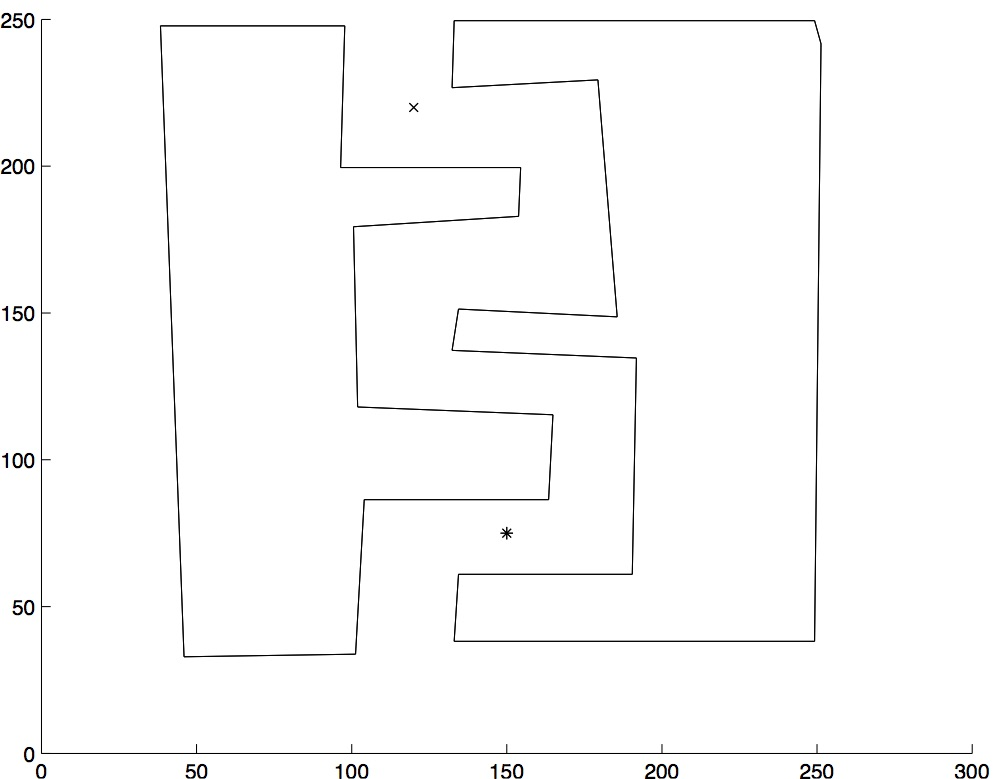
\includegraphics[width=0.8\linewidth]{polygonalMap}
\caption{The map that the units had to navigate through}
\label{fig:histogram}
\end{figure}

\subsection{Results}
The strategy described in the previous chapters worked perfectly fine for the simpler models such as the point models, and even the shorter car models.
Thousands of possible paths could be generated within a short period of time.
The best ones of these randomly generated paths were very close to the results of the other groups that did well.
However, when it came to the car models with lenghts of $ >30$, the algorithm could not find any paths at all, even when it was allowed to run for hours.

\begin{table}
    \begin{tabular}{llllllllll}
    ~   & P11a  & P11b       & P12a  & P12b  & P13a    & P13b     & P14a          & P14b  & P15a        \\
    G1  & 16.8  & 26.9(R=30) & 10.3  & 30.2  & ~       & 312      & 27.9          & 11.5  & ~           \\
    G2  & 13.5  & 33.3       & 11.8  & 23.3  & 54.80   & 51.62    & -             & -     & -           \\
    G3  & 17.1  & 34         & 13    & 19    & 48      & 34 (L=1) & 74.2          & 32.4  & 77.9        \\
    G4  & 17.2  & 40.8       & 30    & 28    & ~       & ~        & \\    61\\    & 79    & 170         \\
    G5  & 16    & 36.8       & 45    & ~     & 98.1    & ~        & 77.61         & ~     & 168.72      \\
    G6  & 15.6  & ~          & ~     & 37.7  & > 8 min & 61.4     & 38.5          & 28.5  & ~           \\
    G7  & 16.3  & 21.22      & 11.1  & ~     & 72.02   & ~        & 28.84         & 12.44 & 238.24      \\
    G8  & 23    & 40         & 53    & ~     & 71.83   & 89.92    & 43            & 36.24 & ~           \\
    G9  & 10.89 & 19.03      & 5.76  & 26.00 & 57.56   & 28.90    & 27.45         & 10.04 & 96.6        \\
    G10 & 12.28 & 20.16      & ~     & 25.00 & 68.5    & 53.9     & 49.3          & 22.2  & 163.5       \\
    G11 & 14.4  & 15.5       & 12.6  & 20.3  & 46.8    & 28.3     & 29.3          & 15.3  & 41.6 (min)  \\
    G12 & 18.38 & 30.42      & 37.18 & 30.12 & 72.72   & 50.64    & 61.60         & 20.54 & 193.08      \\
    G13 & 15.38 & 54         & 44    & ~     & 353     & ~        & 63            & 23    & ~           \\
    ~   & ~     & ~          & ~     & ~     & ~       & ~        & ~             & ~     & ~           \\
    \end{tabular}
\end{table}
\pagebreak
%%%%%%%%%%%%%%%%%%%%%%%%%%%%%%%%%%%%%%%%%%%%%%%%%%%%%%%%%%%%%
%%%%%%%%%%%%%%%%%%%%%%%%%%%%%%%%%%%%%%%%%%%%%%%%%%%%%%%%%%%%%
\section{Summary and Conclusions}
\label{sec:summary}
\subsection{Summary}
In summary, we tried to navigate units with different motion models, including dynamic point, dynamic car and kinematic car with the help of RRT. The paths that RRT generated, were random and therefore likely to be sub-optimal. However, due to the speed of which they were generated, we were allowed to create a great number of possible paths and pick the best one.
In most cases, this proved to be a sufficient strategy. However, when it came to cases where extreme precission was required, such as in cases where large vehicles need to navigate through small spaces, the model did not perform well.
\subsection{Conclusions}
The strategy that we adopted in our implementation proved to be successful for the test cases where precision was not vital in order to reach a goal.
In these cases, the probability of randomly arriving to the circumstances that was required for the unit to be able to traverse a choke point proved to be too small with our heuristics.
This is almost to be expected, since the main purpose of our heuristics were to spread the tree rapidly in all directions without showing too much concern for the final goal destination.
The algorithm finally turns its attention towards a goal when the goal node has been spotted. But by then, the circumstances of the node that spotted the goal, such as its position, speed and angle would usually prevent it from being able to reach the goal node. 

Group 11, which also used a plain RRT algorithm were more successful with their implementation. Their strategy was the same as our initial strategy of sampling the goal node with a certain frequency. However, they resolved the issue of the tree getting convoluted by branches that “crashed” into the obstacles by performing moves in chains of 10, and then discarding the entire chain if it crashed into an obstacle.
This was a better strategy than ours since this solved the issue of convoluted trees with redundant and unusable branches, while still retaining the advantage of focusing towards the goal during the entire running time of the algorithm.

%%%%%%%%%%%%%%%%%%%%%%%%%%%%%%%%%%%%%%%%%%%%%%%%%%%%%%%%%%%%%
%%%%%%%%%%%%%%%%%%%%%%%%%%%%%%%%%%%%%%%%%%%%%%%%%%%%%%%%%%%%%
\pagebreak
\bibliography{reflist}{}
\bibliographystyle{plain}


\end{document}